%!TEX root = ../username.tex
\chapter{Introduction} \label{sec:introduction}

When comparing the human brain to machines, humans are better at interpreting data at a higher level and in a more abstract format, whereas machines excel in processing raw numerical data due to their high computational power. Additionally, by Moore's law, the number of transistors in a dense integrated circuit doubles every two years, leading to machines becoming more powerful over the year. Hence, if machines can interpret and understand the representation of objects beyond raw numerical data, they can process and react much faster than humans. Machine vision proves advantageous to humans in situations that require quick reactions, such as in everyday traffic. If executed correctly, machines equipped with vision can predict and prevent traffic accidents faster than humans, thus facilitating safer traffic flow.

Over the last decade, we have seen multiple raised startups, as well as big corporations, pour millions of dollars into research to try to obtain a piece of the autonomous vehicle market which is valued at billions of dollars \cite{autonomous_vehicle_market}. One of the leading companies in the field of autonomous vehicles is Tesla. In October 2015, Tesla released the Tesla Version 7.0 software enabling the Autopilot feature for the Model S and promised that the car would be fully autonomous in 2017 \cite{tesla_software_v7, tesla_2017_promise}. However, in July 2022, 2 different Tesla cars crashed while on autopilot, and each crash caused the death of a motorcyclist \cite{tesla_crash2}. Additionally, in 2019, a Tesla autopilot crashed into a Honda Civic and killed two people \cite{tesla_crash1}. Not to mention, there are 273 Tesla crashes involving the autopilot system reported just in 2019 \cite{autonomous_vehicle_market}. As we can see, as of 2022, we have yet to be able to develop a fully autonomous system.

To be able to achieve a fully autonomous vehicle, it is crucial to identify which module or modules in the autonomous driving modular pipeline are at fault. The autonomous driving modular pipeline consists of four components. These components are Perception and Localization, High-Level Path Planning, Behavior Arbitration, and Motion Controllers [Fig. \ref{fig:autonomous_driving_pipeline}].

\begin{figure}[!ht] \centering
    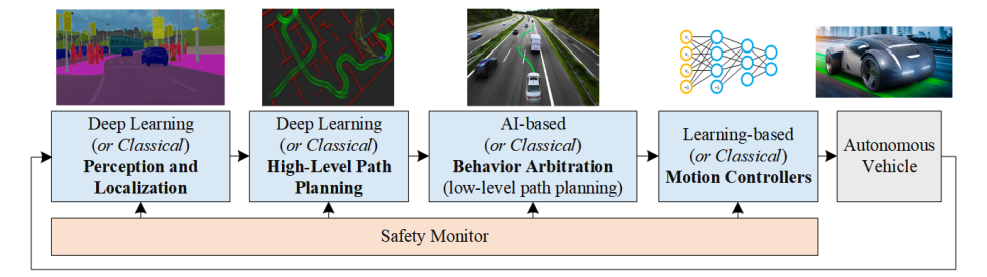
\includegraphics[keepaspectratio=true,width=6in]{figures/autonomous_driving_modular_pipeline.png}
    \caption{Deep Learning Based Autonomous Driving Modular Pipeline \cite{grigorescu_trasnea_cocias_macesanu_2020}}
    \label{fig:autonomous_driving_pipeline}
\end{figure}

To identify which module or modules are at fault, we need to understand and analyze each module of the modular pipeline. In this paper, we will only look at Perception and Localization, the first module in the autonomous vehicle pipeline. The Perception and Localization module is responsible for answering two questions: "Where is the car?" and "What is around the car?" \cite{liu_2020}. To perform this function, the module utilizes the sensing hardware and the software to understand the scene. Such hardware includes LiDAR, cameras, and other sensors. Nonetheless, they are all used for getting the information surrounding the vehicle and feeding those data to the software functionality of the module.

In this study, we assume that the sensor (hardware) is reliable and able to pass the surrounding data to the software part of the module. With the recorded data, the software module must be able to understand the data scene, which is a very challenging task. Unlike human beings, machine sees and processes objects differently from our eyes and brain. While we see the object as a whole, the machine sees it as a grid of values that do not have any connection with one another. For this reason, the Computer Vision field tackles this problem and tries to create algorithms that are able to make sense of the object representation beyond the raw numerical data. The most important groups of algorithms in the Computer Vision field for understanding traffic scenes are video segmentation algorithms.

There are two types of video segmentation algorithms. The two are video semantic segmentation and video instance segmentation. In the video semantic segmentation algorithm, for each scene, objects in the scene are grouped and classified based on categories \cite{overview_cv_task}. On the other hand, video instance segmentation detects each instance of each category for each scene \cite{overview_cv_task}. Comparing semantic segmentation and instance segmentation, we can see that instance segmentation proposes a higher accuracy and detail as it is able to see each instance of a class. That is, the instance segmentation algorithm will be able to distinguish between a car and another car behind it, while semantic segmentation considers these two cars as one. Further discussion of semantic segmentation and instance segmentation is provided in Section \ref{sec:cv_tasks}.

Since video instance segmentation algorithms give higher detection accuracy, in this paper, we assume an algorithm from this group is used for the Perception and Localization module. Knowing a video is a sequence of images, many video instance segmentation algorithms were proposed based on an algorithm in image instance segmentation. One example of such an algorithm is MaskTrack R-CNN which includes a new tracking branch to the well-known image instance segmentation Mask R-CNN. For that reason, to understand video instance segmentation, we first need to understand and analyze image instance segmentation which is adapted from an object detection model. More specifically, this paper discusses the building blocks of the object detection model and its application in image segmentation tasks. We analyze and compare the performance of two well-known algorithms, the Mask R-CNN and You Only Look Once version 5 (YOLOv5), in the object detection task. Furthermore, we want to identify if failure to detect objects by these image object detection algorithms causes the autonomous driving pipeline to fail and result in accidents.
